%%%%%%%%%%%%%%%%%%%%%%%%%%%%%%%%%%%%%%%%%
% Jacobs Landscape Poster
% LaTeX Template
% Version 1.0 (29/03/13)
%
% Created by:
% Computational Physics and Biophysics Group, Jacobs University
% https://teamwork.jacobs-university.de:8443/confluence/display/CoPandBiG/LaTeX+Poster
% 
% Further modified by:
% Nathaniel Johnston (nathaniel@njohnston.ca)
%
% This template has been downloaded from:
% http://www.LaTeXTemplates.com
%
% License:
% CC BY-NC-SA 3.0 (http://creativecommons.org/licenses/by-nc-sa/3.0/)
%
%%%%%%%%%%%%%%%%%%%%%%%%%%%%%%%%%%%%%%%%%

%----------------------------------------------------------------------------------------
%	PACKAGES AND OTHER DOCUMENT CONFIGURATIONS
%----------------------------------------------------------------------------------------

\documentclass[final]{beamer}

\usepackage[scale=1.24]{beamerposter} % Use the beamerposter package for laying out the poster
%\usepackage{enumitem}
%\setlist{nosep}
\usetheme{confposter} % Use the confposter theme supplied with this template

\setbeamercolor{block title}{fg=ngreen,bg=white} % Colors of the block titles
\setbeamercolor{block body}{fg=black,bg=white} % Colors of the body of blocks
\setbeamercolor{block alerted title}{fg=ucdgold,bg=ucdblue} % Colors of the highlighted block titles
\setbeamercolor{block alerted body}{fg=black,bg=dblue!10} % Colors of the body of highlighted blocks
% Many more colors are available for use in beamerthemeconfposter.sty

%-----------------------------------------------------------
% Define the column widths and overall poster size
% To set effective sepwid, onecolwid and twocolwid values, first choose how many columns you want and how much separation you want between columns
% In this template, the separation width chosen is 0.024 of the paper width and a 4-column layout
% onecolwid should therefore be (1-(# of columns+1)*sepwid)/# of columns e.g. (1-(4+1)*0.024)/4 = 0.22
% Set twocolwid to be (2*onecolwid)+sepwid = 0.464
% Set threecolwid to be (3*onecolwid)+2*sepwid = 0.708

\newlength{\sepwid}
\newlength{\onecolwid}
\newlength{\twocolwid}
\newlength{\threecolwid}
\newlength{\fourcolwid}
\setlength{\paperwidth}{48in} % A0 width: 46.8in
\setlength{\paperheight}{36in} % A0 height: 33.1in
\setlength{\sepwid}{0.024\paperwidth} % Separation width (white space) between columns
\setlength{\onecolwid}{0.24\paperwidth} % Width of one column
\setlength{\twocolwid}{0.424\paperwidth} % Width of two columns
\setlength{\threecolwid}{0.708\paperwidth} % Width of three columns
\setlength{\fourcolwid}{0.952\paperwidth}
\setlength{\topmargin}{-0.5in} % Reduce the top margin size
%-----------------------------------------------------------

\usepackage{graphicx}  % Required for including images
\usepackage{graphics}
\usepackage{booktabs} % Top and bottom rules for tables

%----------------------------------------------------------------------------------------
%	TITLE SECTION 
%----------------------------------------------------------------------------------------

\title{TempestExtremes BlobMetrics: An R-based analysis toolkit for\\ assessment and intercomparison of atmospheric blocking datasets} % Poster title

\author{M.C. Pinheiro,\texorpdfstring{$^1$}, P.A. Ullrich,\texorpdfstring{$^{1,2}$}, R. Grotjahn\texorpdfstring{$^1$}. }

\institute{1. University of California, Davis 2. Lawrence Berkeley National Laboratory} % Institution(s)

%----------------------------------------------------------------------------------------

\setbeamertemplate{headline}{
 \leavevmode
  \begin{columns}[b]
   \begin{column}{.08\linewidth}
   %\vspace{10em}
          %
\includegraphics[width=\linewidth]{nasa_logo}\\
          %\vspace{2em}
       %
\includegraphics[width=1.6\linewidth]{uc_logo}
       
\includegraphics[width=\linewidth]{nasa_logo}
       \vspace{1.2em}
   \end{column}
   \begin{column}{.83\linewidth}
    \vskip1cm
    \centering
    \usebeamercolor{title in headline}{\color{jblue}\Huge{\textbf{\inserttitle}}\\[0.5ex]}
    \usebeamercolor{author in headline}{\color{fg}\Large{\insertauthor}\\[1ex]}
    \usebeamercolor{institute in headline}{\color{fg}\large{\insertinstitute}\\[1ex]}
    \vskip1cm
   \end{column}
   \begin{column}{.09\linewidth}
        %\vspace{-0.5em}
          %
\includegraphics[width=.75\linewidth]{doe_logo}\\
          %\vspace{0.75em}
       %
\includegraphics[width=.75\linewidth]{lbl_logo}
       %\vspace{8em}
       \hspace{-6em}
        
\includegraphics[width=1.3\linewidth]{uc_logo}
      %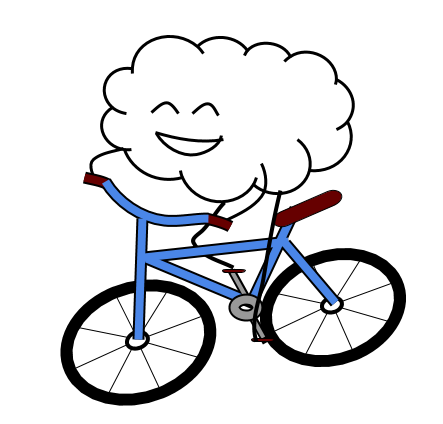
\includegraphics[width=.75\linewidth]{cloud_bike.png}
       \vspace{2em}
   \end{column}
   %\vspace{1cm}
  \end{columns}
 %\vspace{0.5in}
 \hspace{0.5in}\begin{beamercolorbox}[wd=47in,colsep=0.15cm]{cboxb}\end{beamercolorbox}
 %\vspace{0.1in}
}

\begin{document}

\addtobeamertemplate{block end}{}{\vspace*{2ex}} % White space under blocks
\addtobeamertemplate{block alerted end}{}{\vspace*{2ex}} % White space under highlighted (alert) blocks

\setlength{\belowcaptionskip}{2ex} % White space under figures
\setlength\belowdisplayshortskip{2ex} % White space under equations

\begin{frame}[t] % The whole poster is enclosed in one beamer frame
\vspace{-3em}
\begin{columns}[t] % The whole poster consists of three major columns, the second of which is split into two columns twice - the [t] option aligns each column's content to the top
\begin{column}{\sepwid}\end{column} % Empty spacer column
\begin{column}{\fourcolwid}

\begin{exampleblock}{}
\small{Objective blocking detection algorithms make it possible to analyze blocking patterns on extremely high volumes of data, which makes it ideal for efficiently assessing blocking patterns across many potential future climate scenarios. However, block detection is highly dependent on the algorithm, season, and region of study; agreement on averaged blocking patterns does not guarantee that results are similar in terms of block characteristics such as block size, duration, or location (Pinheiro et al, pending). Therefore, it is important to assess blocking in terms of distinct features rather than on a per-gridpoint basis. The StitchBlobs analysis tool in the TempestExtremes package allows users to assess blocking patterns from a given input dataset, providing information for each unique block. BlobMetrics, a new R-based analysis framework, adds additional functionality to the existing StitchBlobs tool. BlobMetrics provides both per-timestep and summarized per-block information on block characteristics, as well as the capability to compare results from multiple blocking detection algorithms. }
\end{exampleblock}
%\vspace{-1em}
\end{column}
\begin{column}{\sepwid}\end{column} % Empty spacer column
\end{columns}
\begin{columns}[t]
%----------------------------------------------------------------
%SPACER
%---------------------------------------------------------------
\begin{column}{\sepwid}\end{column} % Empty spacer column
%---------------------------------------------------------------
%LEFT COLUMN
%-------------------------------------------------------------------
\begin{column}{\onecolwid} % The first column
%----------------------------------------------------------------------------------------
%	OVERVIEW
%----------------------------------------------------------------------------------------



\begin{alertblock}{Motivation}
Objective detection of blocking algorithms can depend on the algorithm or model
\begin{itemize}
    \item Per-timestep: timing, size, location
    \item seasonal average: percentage of blocked days, 
    \item can affect attempts to correlate blocking with extreme weather
\end{itemize}
\begin{figure}
    \centering
    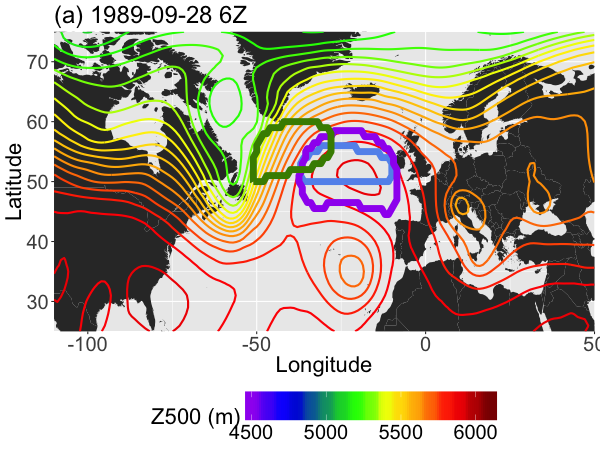
\includegraphics[width=\textwidth]{fig8a.png}
    \caption{Omega block detected by three separate objective detection algorithms (source: Pinheiro et al 2019 (under review))}
    \label{fig:block_compare}
\end{figure}
\vspace{-1.5em}
    \begin{itemize}
        \item \textbf{Possible comparisons:}
        \begin{itemize}
            \item Different detection algorithms
            \item Different reanalyses
            \item Reanalysis vs model results
        \end{itemize}
    \end{itemize}

\end{alertblock}
\begin{block}{References}

\nocite{*} % Insert publications even if they are not cited in the poster
\small{\bibliographystyle{unsrt}
\bibliography{sample}\vspace{0.75in}}
\end{block}
\begin{block}{Acknowledgments}
\small{US DOE Office of Science award DE-SC0016605, and USDA NIFA Hatch project Accession \#1010971}
\end{block}

%----------------------------------------------------------------------------------------

\end{column} % End of the first column

\begin{column}{\sepwid}\end{column} % Empty spacer column

%\begin{column}{\twocolwid} % Begin a column which is two columns wide (column 2)
\begin{column}{\twocolwid}
%----------------------------------------------------------------------------------------
%	SCHEMATIC
%----------------------------------------------------------------------------------------
%\begin{minipage}[t]{0.6\textwidth}
\begin{figure}
    \centering
    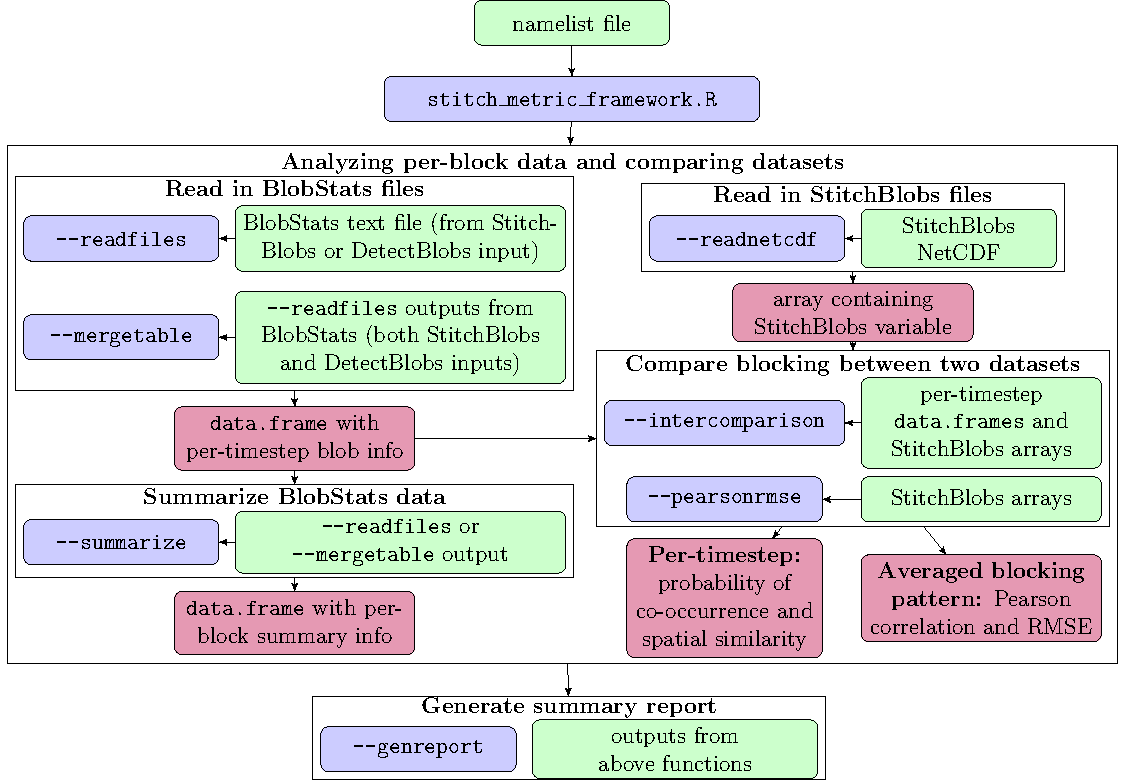
\includegraphics[width=0.9\textwidth]{Framework_figure.pdf}
    \caption{Schematic of BlobMetrics. Input files are green, analysis tools are purple, and output files are pink. }
    \label{fig:Blobfig}
\end{figure}
%\end{minipage}
%\begin{minipage}[t]{0.39\textwidth}

%\end{minipage}
\begin{block}{Example Output}

\begin{table}
\resizebox{0.7\columnwidth}{!}{
\begin{tabular}{l|l|l|l|l|l}
\hline
  & CMCC-CESM & JRA & MERRA & CFSR & ERA\\
\hline
Number of unique blobs & 141 & 127 & 119 & 126 & 126\\
\hline
Number of merged blobs & 32 & 48 & 44 & 47 & 46\\
\hline
Maximum blocking frequency & 0.2462 & 0.2160 & 0.1918 & 0.1870 & 0.1991\\
\hline
Interquartile range of blob centroid lat & 37.11 53.81 & 36.25 51.88 & 36.75 52.00 & 37.00 52.00 & 36.00 51.50\\
\hline
Number of blocked days & 1539 & 1526 & 1468 & 1473 & 1531\\
\hline
Average number of blocked days & 61.56 & 61.04 & 58.72 & 58.92 & 61.24\\
\hline
Interquartile range of duration (days) & 6.00 15.00 & 7.12 15.25 & 7.25 15.50 & 7.06 14.44 & 7.25 14.94\\
\hline
Interquartile range of speed (km/hr) & 2.78 11.55 & 2.13 12.90 & 2.89 13.43 & 3.97 15.37 & 2.88 13.17\\
\hline
Interquartile range of blob size (10\textasciicircum{}6 km\textasciicircum{}2) & 3.1 8.3 & 3.2 7.9 & 3.2 7.9 & 3.2 7.8 & 3.2 7.9\\
\hline
\end{tabular}
}
\caption{Summary statistics for CMCC-CESM, ERA-Interim, MERRA-2, CFSR, and JRA for 1980-2004}
\end{table}
\begin{figure}
    \centering
    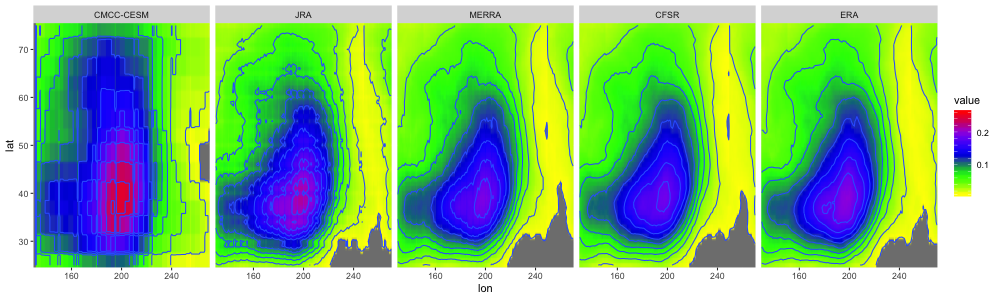
\includegraphics[width=0.65\textwidth]{freq.png}
    \caption{Blocking frequency for winter (DJF) in NH Pacific, 1980-2004}
    \label{fig:freq}
\end{figure}

\end{block}

\end{column} % End of the second column

\begin{column}{\sepwid}\end{column} % Empty spacer column

 \begin{column}{\onecolwid} % The third column

\begin{alertblock}{BlobMetrics Overview}
\begin{itemize}
    \item \textbf{BlobMetrics} is an R-based analysis framework that summarizes blocking data and generates an output report in HTML format
    \item New tool in the existing \textbf{TempestExtremes} analysis framework \cite{ullrich_tempestextremes:_2017}
    \begin{itemize}
        \item \textbf{StitchBlobs} tool tracks gridpoint clusters across space and time; results are individually tagged objects in NetCDF file
       \item \textbf{DetectBlobs} tracks gridpoint clusters without joining them across the time axis
        \item \textbf{BlobStats} tool takes StitchBlobs NetCDF and provides per-timestep text summary of each object's size, extent, and centroid coordinates
        \item BlobMetrics takes the above outputs and generates summary statistics on individual block characteristics 
    \end{itemize}
\end{itemize}
\textbf{Minimum requirements:}\\
\begin{minipage}[h]{0.73\textwidth}
\begin{itemize}
    \item StitchBlobs and BlobStats output
    \item R software and libraries 
    \item NetCDF libraries
\end{itemize}
\end{minipage} 
\begin{minipage}[h]{0.25\textwidth}
\begin{figure}
    \centering

\includegraphics[width=\textwidth]{frame.png}
%\caption{Scan here for link to TempestExtremes}
    \label{fig:qr}
\end{figure}
\end{minipage}
\textbf{Future implementation:}
\begin{itemize}
    \item Reanalysis/model comparison report template
    \item magnitude of Z500 in detected blocks
\end{itemize}
\end{alertblock}
\begin{figure}
    \centering
    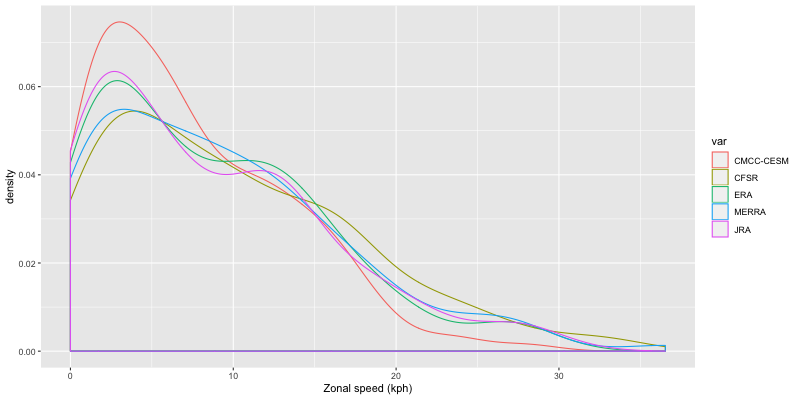
\includegraphics[width=0.9\textwidth]{speed_dist.png}\\
    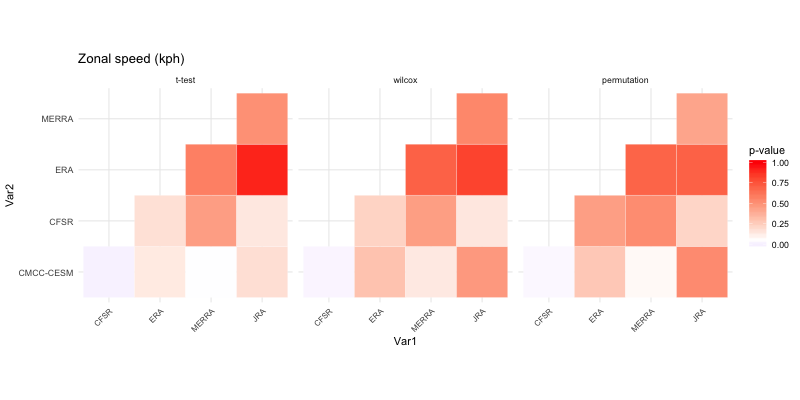
\includegraphics[width=0.8\textwidth]{speed_pvalue.png}
    \caption{Distributions of block speed(top) and p-value for  }
    \label{fig:pval_dist}
\end{figure}

% %----------------------------------------------------------------------------------------
% %	REFERENCES
% %----------------------------------------------------------------------------------------



% %----------------------------------------------------------------------------------------
% %	ACKNOWLEDGEMENTS
% %----------------------------------------------------------------------------------------

% \setbeamercolor{block title}{fg=red,bg=white} % Change the block title color

% \begin{block}{Acknowledgements}

% \small{\rmfamily{Nam mollis tristique neque eu luctus. Suspendisse rutrum congue nisi sed convallis. Aenean id neque dolor. Pellentesque habitant morbi tristique senectus et netus et malesuada fames ac turpis egestas.}} \\

% \end{block}

% %----------------------------------------------------------------------------------------
% %	CONTACT INFORMATION
% %----------------------------------------------------------------------------------------

% % \setbeamercolor{block alerted title}{fg=black,bg=norange} % Change the alert block title colors
% % \setbeamercolor{block alerted body}{fg=black,bg=white} % Change the alert block body colors

% % \begin{alertblock}{QR CODE HERE}

% % \begin{itemize}
% % \item Web: \href{http://www.university.edu/smithlab}{http://www.university.edu/smithlab}
% % \item Email: \href{mailto:john@smith.com}{john@smith.com}
% % \item Phone: +1 (000) 111 1111
% % \end{itemize}

% % \end{alertblock}

% %----------------------------------------------------------------------------------------

 \end{column} % End of the third column

\end{columns} % End of all the columns in the poster

\end{frame} % End of the enclosing frame

\end{document}
